% ==== Data Analytics Foundations =============================================================================
\chapter{Data Analytics Foundations}

% ---- 4.1 Data Preprocessing -------------------------------------------------------------------------
\section{Data Preprocessing}

% ---- 4.1.1 Data Cleaning ----------------------------------------------------------------------------
\subsection{Data Cleaning}

\begin{tcbitemize}[ skin=sectionraster ]
    \tcbitem[title=Why Data Cleaning?, raster multicolumn=3]
    Real-world data is rarely clean: values may be missing, erroneous, duplicated, or inconsistent.
    Data cleaning (also \emph{data scrubbing}) identifies and corrects these issues before any analysis\textsuperscript{\cite{hanDataMiningConcepts2012}}.
    Garbage in, garbage out: dirty data systematically corrupts model outputs.
    \tcblower
    \begin{itemize}
        \item \textbf{Incompleteness}: missing attributes or records
        \item \textbf{Noise}: random error or variance in values
        \item \textbf{Inconsistency}: conflicting codes or names
        \item \textbf{Duplicates}: same entity recorded multiple times
    \end{itemize}

    \tcbitem[title={Missing Data: MCAR, MAR, MNAR}, raster multicolumn=3]
    Rubin (1976) classified missingness into three mechanisms\textsuperscript{\cite{brucePracticalStatisticsData2017}}:
    \tcblower
    \begin{tblr}{colspec={|Q[l,m,2cm]|X|}, hlines}
        \textbf{Type} & \textbf{Meaning} \\
        MCAR & Missing Completely At Random — missingness is independent of all data \\
        MAR  & Missing At Random — missingness depends on observed data only \\
        MNAR & Missing Not At Random — missingness depends on the unobserved value itself \\
    \end{tblr}
\captionof{table}{Data Cleaning: Missing Data: MCAR, MAR, MNAR.}
\label{tab:ch04-data-analytics-inline-01}

    \tcbitem[title=Outlier Detection, raster multicolumn=3]
    Outliers are observations that deviate markedly from the overall pattern\textsuperscript{\cite{hanDataMiningConcepts2012}}.
    Two classical rules for univariate detection:
    \tcblower
    \textbf{IQR rule}: flag $x$ if $x < Q_1 - 1.5\,\mathrm{IQR}$ or $x > Q_3 + 1.5\,\mathrm{IQR}$, where $\mathrm{IQR} = Q_3 - Q_1$.

    \textbf{Z-score rule}: flag $x$ if $|z| > 3$, where
    \begin{equation}
        z = \frac{x - \mu}{\sigma}
    \end{equation}
    Multivariate outliers require distance-based methods (Mahalanobis) or density-based methods (LOF).

    \tcbitem[title=Imputation Strategies, raster multicolumn=3]
    Imputation replaces missing values with plausible substitutes rather than discarding whole records\textsuperscript{\cite{brucePracticalStatisticsData2017}}.
    \tcblower
    \begin{tblr}{colspec={|X|X|}, hlines}
        \textbf{Strategy} & \textbf{Notes} \\
        Mean / median      & Simple; distorts variance \\
        Mode (categorical) & Assigns most frequent class \\
        Forward/back fill  & Time series; propagates last known value \\
        k-NN imputation    & Uses similar records; better for MAR \\
        Model-based (MICE) & Multiple Imputation by Chained Equations; commonly relies on a Missing At Random assumption, while MNAR requires explicit sensitivity or missingness modelling \\
    \end{tblr}
\captionof{table}{Data Cleaning: Imputation Strategies.}
\label{tab:ch04-data-analytics-inline-02}
\end{tcbitemize}

% ---- 4.1.2 Data Integration -------------------------------------------------------------------------
\subsection{Data Integration}

\begin{tcbitemize}[ skin=sectionraster ]
    \tcbitem[title={Schema Matching \& Entity Resolution}, raster multicolumn=3]
    When merging data from multiple sources, \emph{schema matching} maps attributes from one source to semantically equivalent attributes in another\textsuperscript{\cite{hanDataMiningConcepts2012}}.
    \emph{Entity resolution} (record linkage) identifies records that refer to the same real-world entity despite differences in representation (e.g., ``J. Smith'' vs.\ ``John Smith'').
    \tcblower
    \begin{itemize}
        \item Similarity metrics: Jaccard, edit distance, phonetic codes
        \item Blocking: candidate-pair reduction to avoid $O(n^2)$ comparisons
        \item Deterministic rules vs.\ probabilistic scoring
    \end{itemize}

    \tcbitem[title={ETL Pipelines}, raster multicolumn=3]
    \textbf{Extract--Transform--Load} is the standard pattern for moving data into a data warehouse or analytical store\textsuperscript{\cite{hanDataMiningConcepts2012}}.
    \tcblower
    \begin{tblr}{colspec={|Q[c,m,1.2cm]|X|}, hlines}
        \textbf{Step}   & \textbf{Description} \\
        Extract  & Pull raw data from operational sources (databases, APIs, files) \\
        Transform & Clean, reshape, aggregate, apply business rules \\
        Load     & Write to target (DW, data lake, OLAP cube) \\
    \end{tblr}
\captionof{table}{Data Integration: ETL Pipelines.}
\label{tab:ch04-data-analytics-inline-03}
    Modern \emph{ELT} (load first, transform in-place) is preferred for cloud data lakes where storage is cheap and compute is elastic.

    \tcbitem[title=Data Fusion, raster multicolumn=6]
    Data fusion combines information from heterogeneous sources to produce a more complete or accurate dataset than any single source provides alone\textsuperscript{\cite{hanDataMiningConcepts2012}}.
    Challenges include conflicting values (\emph{data conflicts}), different granularities (\emph{data aggregation mismatch}), and temporal drift (sources updated at different frequencies).
    Resolution strategies range from source trust ranking and majority voting to probabilistic graphical models that jointly estimate the true value.
\end{tcbitemize}

% ---- 4.1.3 Data Transformation ----------------------------------------------------------------------
\subsection{Data Transformation}

\begin{tcbitemize}[ skin=sectionraster ]
    \tcbitem[title=Min-Max Normalization, raster multicolumn=3]
    Rescales values to a fixed interval $[a, b]$, typically $[0, 1]$\textsuperscript{\cite{hanDataMiningConcepts2012}}.
    Preserves the original distribution shape but is sensitive to outliers.
    \begin{equation}
        x' = \frac{x - x_{\min}}{x_{\max} - x_{\min}}(b - a) + a
    \end{equation}

    \tcbitem[title=Z-Score Standardization, raster multicolumn=3]
    Centers and scales to zero mean and unit variance\textsuperscript{\cite{hanDataMiningConcepts2012}}.
    Preferred when the distribution is approximately normal or when the algorithm is sensitive to scale (SVMs, PCA, gradient descent).
    \begin{equation}
        x' = \frac{x - \mu}{\sigma}
    \end{equation}
    After standardization: $\mathbb{E}[x'] = 0$, $\mathrm{Var}(x') = 1$.

    \tcbitem[title=Categorical Encoding, raster multicolumn=3]
    Algorithms typically require numerical input; categorical variables must be encoded\textsuperscript{\cite{molinHandsonDataAnalysis2021}}.
    \tcblower
    \begin{tblr}{colspec={|X|X|}, hlines}
        \textbf{Encoding}    & \textbf{When to use} \\
        One-hot (dummy)       & Nominal; no ordinal relationship; creates $k$ binary columns \\
        Label encoding        & Ordinal or tree-based models where ordering is irrelevant \\
        Target encoding       & High-cardinality nominals; replaces category with mean target value \\
        Binary / Hash trick   & Very high cardinality; reduces dimensionality at cost of collisions \\
    \end{tblr}
\captionof{table}{Data Transformation: Categorical Encoding.}
\label{tab:ch04-data-analytics-inline-04}

    \tcbitem[title=Log and Power Transforms, raster multicolumn=3]
    Highly skewed features violate the normality assumptions of many models and can dominate distance metrics\textsuperscript{\cite{hanDataMiningConcepts2012}}.
    \tcblower
    \begin{itemize}
        \item $\log(x + 1)$: compresses right-skewed data (counts, prices)
        \item Square-root: moderate skew, preserves zeros
        \item Box--Cox: parametric family $x^{(\lambda)} = \frac{x^\lambda - 1}{\lambda}$; $\lambda$ estimated from data
        \item Yeo--Johnson: extends Box--Cox to negative values
    \end{itemize}
\end{tcbitemize}

% ---- 4.1.4 Data Reduction ---------------------------------------------------------------------------
\subsection{Data Reduction}

\begin{tcbitemize}[ skin=sectionraster ]
    \tcbitem[title={Feature Selection vs. Feature Extraction}, raster multicolumn=3]
    Both reduce dimensionality, but differ in approach\textsuperscript{\cite{hanDataMiningConcepts2012}}.
    \tcblower
    \begin{tblr}{colspec={|X|X|}, hlines}
        \textbf{Feature Selection} & \textbf{Feature Extraction} \\
        Selects a subset of original features & Creates new features from originals \\
        Preserves interpretability & May lose interpretability \\
        Filter, Wrapper, Embedded methods & PCA, autoencoders, LDA \\
        No transformation of values & Projects data into new space \\
    \end{tblr}
\captionof{table}{Data Reduction: Feature Selection vs. Feature Extraction.}
\label{tab:ch04-data-analytics-inline-05}

    \tcbitem[title={PCA: Principal Component Analysis}, raster multicolumn=3]
    PCA finds orthogonal directions (principal components) of maximum variance in the data\textsuperscript{\cite{hastieElementsStatisticalLearning2008}}.
    Components are eigenvectors of the covariance matrix $\mathbf{C} = \frac{1}{n}\mathbf{X}^\top\mathbf{X}$, ordered by descending eigenvalue.
    Projecting onto the top-$k$ components minimizes reconstruction error under the Frobenius norm.
    \begin{equation}
        \mathbf{Z} = \mathbf{X}\mathbf{W}_k, \quad \mathbf{W}_k \in \mathbb{R}^{d \times k}
    \end{equation}

    \tcbitem[title=Sampling Strategies, raster multicolumn=6]
    When full-data computation is infeasible, sampling produces a representative subset\textsuperscript{\cite{hanDataMiningConcepts2012}}.
    \tcblower
    \begin{tblr}{colspec={|X|X|X|}, hlines}
        \textbf{Method}           & \textbf{How}                                    & \textbf{Use case} \\
        Simple random             & Each record drawn with equal probability         & General baseline \\
        Stratified                & Draw proportionally from each stratum            & Imbalanced classes \\
        Cluster                   & Select clusters, then sample within              & Geographically distributed data \\
        Systematic                & Every $k$-th record                              & Ordered datasets \\
        Reservoir (online)        & Fixed-size sample from a stream in one pass      & Streaming / big data \\
    \end{tblr}
\captionof{table}{Data Reduction: Sampling Strategies.}
\label{tab:ch04-data-analytics-inline-06}
\end{tcbitemize}

% ---- 4.1.5 Foundations of Data Systems --------------------------------------------------------------
\subsection{Foundations of Data Systems}

\subsubsection{Reliability}

\begin{tcbitemize}[ skin=sectionraster ]
    \tcbitem[title=Reliability in Data Systems, raster multicolumn=3]
    A reliable system continues to work correctly even when faults occur\textsuperscript{\cite{gujaStartingDataAnalytics2025}}.
    A \emph{fault} (one component misbehaves) must be distinguished from a \emph{failure} (the whole system stops delivering its service).
    Systems are made fault-tolerant by tolerating faults before they escalate to failures.
    \tcblower
    \begin{itemize}
        \item \textbf{Hardware faults}: RAID disks, dual power, hot standby
        \item \textbf{Software faults}: extensive testing, process isolation, chaos engineering
        \item \textbf{Human faults}: administrative interfaces with guard rails, easy rollback, monitoring
    \end{itemize}

    \tcbitem[title={MTBF, MTTR, Availability}, raster multicolumn=3]
    Reliability is quantified using failure-rate metrics\textsuperscript{\cite{gujaStartingDataAnalytics2025}}.
    \begin{equation}
        \text{Availability} = \frac{\text{MTBF}}{\text{MTBF} + \text{MTTR}}
    \end{equation}
    \begin{itemize}
        \item \textbf{MTBF} — Mean Time Between Failures
        \item \textbf{MTTR} — Mean Time To Recovery
        \item \textbf{SLA} — Service Level Agreement: contractual availability target (e.g., 99.9\% = 8.7 h downtime/year)
        \item \textbf{Redundancy}: $n+1$ or $2n$ hot standbys eliminate single points of failure
    \end{itemize}
\end{tcbitemize}

\subsubsection{Scalability}

\begin{tcbitemize}[ skin=sectionraster ]
    \tcbitem[title={Vertical vs. Horizontal Scaling}, raster multicolumn=3]
    As data volume grows, systems must scale\textsuperscript{\cite{gujaStartingDataAnalytics2025}}.
    \tcblower
    \begin{tblr}{colspec={|X|X|X|}, hlines}
        \textbf{Aspect}    & \textbf{Vertical (Scale Up)} & \textbf{Horizontal (Scale Out)} \\
        Approach   & Bigger machine (more CPU/RAM) & More machines in a cluster \\
        Limit      & Single-node hardware ceiling  & Near-linear with node count \\
        Cost model & Non-linear (premium hardware) & Commodity servers \\
        Failure    & Single point of failure       & Graceful degradation \\
    \end{tblr}
\captionof{table}{Foundations of Data Systems: Vertical vs. Horizontal Scaling.}
\label{tab:ch04-data-analytics-inline-07}

    \tcbitem[title=CAP Theorem, raster multicolumn=3]
    In a distributed system it is impossible to simultaneously guarantee all three of\textsuperscript{\cite{gujaStartingDataAnalytics2025}}:
    \begin{itemize}
        \item \textbf{Consistency} (C): every read returns the most recent write
        \item \textbf{Availability} (A): every request receives a (non-error) response
        \item \textbf{Partition tolerance} (P): the system operates despite network partitions
    \end{itemize}
    Since partitions are unavoidable in real networks, designers must choose between CP and AP systems.
    E.g., HBase (CP), Cassandra (AP), RDBMS in single node (CA).

    \tcbitem[title=Load Balancing, raster multicolumn=6]
    Load balancing distributes incoming requests across multiple servers to prevent any single node from becoming a bottleneck\textsuperscript{\cite{gujaStartingDataAnalytics2025}}.
    Common algorithms: round-robin, least-connections, IP-hash, weighted round-robin.
    A \emph{load balancer} also provides health checks; unhealthy nodes are removed from the pool automatically.
    For data-intensive systems, \emph{data partitioning} (sharding) complements load balancing by splitting the data itself — e.g., consistent hashing ensures minimal data migration when nodes are added or removed.
\end{tcbitemize}

\subsubsection{Maintainability}

\begin{tcbitemize}[ skin=sectionraster ]
    \tcbitem[title=Three Pillars of Maintainability, raster multicolumn=6]
    Kleppmann (2017) identifies three design goals that make systems maintainable over time\textsuperscript{\cite{gujaStartingDataAnalytics2025}}.
    \tcblower
    \begin{tblr}{colspec={|Q[l,m,2.5cm]|X|X|}, hlines}
        \textbf{Property}   & \textbf{Meaning}                                                  & \textbf{Practices} \\
        Operability          & Easy for ops teams to keep running day-to-day                     & Good monitoring, documentation, predictable behavior \\
        Simplicity           & New engineers can understand the system                           & Abstraction, clean APIs, remove accidental complexity \\
        Evolvability         & Easy to adapt to new requirements                                 & Modular design, backward-compatible schemas, CI/CD \\
    \end{tblr}
\captionof{table}{Foundations of Data Systems: Three Pillars of Maintainability.}
\label{tab:ch04-data-analytics-inline-08}
\end{tcbitemize}

% ---- 4.1.6 Data Processing at Scale -----------------------------------------------------------------
\subsection{Data Processing at Scale}

\subsubsection{Batch Processing}

\begin{tcbitemize}[ skin=sectionraster ]
    \tcbitem[title=MapReduce Paradigm, raster multicolumn=3]
    MapReduce (Dean \& Ghemawat, 2004) is a programming model for processing large datasets in parallel across a cluster\textsuperscript{\cite{leskovecMiningMassiveDatasets2014}}.
    The programmer provides two functions; the framework handles data distribution, fault recovery, and aggregation automatically.
    \tcblower
    \begin{enumerate}
        \item \textbf{Map}: each worker applies a function to its input split and emits $(key, value)$ pairs
        \item \textbf{Shuffle \& Sort}: framework groups all values by key across all workers
        \item \textbf{Reduce}: each worker aggregates values for its assigned keys into a final result
    \end{enumerate}

    \tcbitem[title={Hadoop \& Apache Spark}, raster multicolumn=3]
    Hadoop provides a distributed file system (HDFS) and a MapReduce runtime\textsuperscript{\cite{leskovecMiningMassiveDatasets2014}}.
    Apache Spark generalizes MapReduce with in-memory computation on Resilient Distributed Datasets (RDDs), delivering 10--100$\times$ speedups for iterative algorithms.
    \tcblower
    \begin{tblr}{colspec={|X|X|X|}, hlines}
        \textbf{Feature}       & \textbf{Hadoop MR}     & \textbf{Spark} \\
        Computation model      & Disk-based             & In-memory (RDD/DataFrame) \\
        Latency                & High (minutes)         & Low (seconds) \\
        Iterative algorithms   & Painful                & Efficient \\
        Ecosystem              & HDFS, YARN, Hive       & SQL, Streaming, MLlib, GraphX \\
    \end{tblr}
\captionof{table}{Data Processing at Scale: Hadoop \& Apache Spark.}
\label{tab:ch04-data-analytics-inline-09}
\end{tcbitemize}

\subsubsection{Stream and Complex Event Processing}

\begin{tcbitemize}[ skin=sectionraster ]
    \tcbitem[title={Real-Time vs. Near-Real-Time Processing}, raster multicolumn=3]
    Stream processing handles data in motion — records are processed as they arrive rather than accumulated first\textsuperscript{\cite{leskovecMiningMassiveDatasets2014}}.
    \tcblower
    \begin{tblr}{colspec={|X|X|X|}, hlines}
        \textbf{Mode}       & \textbf{Latency}        & \textbf{Examples} \\
        Real-time           & $<$10 ms                & Algorithmic trading, fraud detection \\
        Near-real-time      & Seconds to minutes      & Dashboards, recommendations \\
        Micro-batch         & Seconds (Spark Streaming) & Aggregations with windowing \\
        Batch               & Minutes to hours        & Nightly ETL, model retraining \\
    \end{tblr}
\captionof{table}{Data Processing at Scale: Real-Time vs. Near-Real-Time Processing.}
\label{tab:ch04-data-analytics-inline-10}

    \tcbitem[title={Apache Kafka \& Event-Driven Architecture}, raster multicolumn=3]
    Apache Kafka is a distributed, fault-tolerant, high-throughput message log used as the backbone of event-driven data platforms\textsuperscript{\cite{leskovecMiningMassiveDatasets2014}}.
    \tcblower
    \begin{itemize}
        \item \textbf{Topic}: named channel; producers publish, consumers subscribe
        \item \textbf{Partition}: ordered, immutable log; enables parallelism
        \item \textbf{Consumer group}: each partition consumed by exactly one group member
        \item \textbf{Retention}: replayed from any offset; decouples producers from consumers
        \item \textbf{Exactly-once semantics}: idempotent producers + transactions
    \end{itemize}
\end{tcbitemize}

% ---- 4.1.7 Microservices ---------------------------------------------------------------------------
\subsection{Microservices}

\subsubsection{Introduction to Microservices}

\begin{tcbitemize}[ skin=sectionraster ]
    \tcbitem[title={Monolith vs. Microservices}, raster multicolumn=3]
    A \emph{monolithic} application deploys all functionality as a single unit; a \emph{microservices} architecture decomposes it into small, independently deployable services each owning its own data\textsuperscript{\cite{gujaStartingDataAnalytics2025}}.
    \tcblower
    \begin{tblr}{colspec={|X|X|X|}, hlines}
        \textbf{Aspect}      & \textbf{Monolith}         & \textbf{Microservices} \\
        Deployment unit      & Single artifact           & Many small services \\
        Scaling              & Scale whole app           & Scale per service \\
        Fault isolation      & One bug can crash all     & Failures contained \\
        Development          & Simpler initially         & Requires DevOps maturity \\
        Data storage         & Shared DB                 & DB-per-service \\
    \end{tblr}
\captionof{table}{Microservices: Monolith vs. Microservices.}
\label{tab:ch04-data-analytics-inline-11}

    \tcbitem[title={Benefits \& Trade-offs}, raster multicolumn=3]
    Microservices excel at scale and team autonomy but introduce distributed systems complexity\textsuperscript{\cite{gujaStartingDataAnalytics2025}}.
    \tcblower
    \textbf{Benefits:}
    \begin{itemize}
        \item Independent deployability and technology choice per service
        \item Fine-grained scalability; resilience through isolation
        \item Small, focused teams (Conway's Law alignment)
    \end{itemize}
    \textbf{Trade-offs:}
    \begin{itemize}
        \item Network latency, distributed transactions, observability overhead
        \item Operational complexity: many services to deploy, monitor, and version
    \end{itemize}
\end{tcbitemize}

\subsubsection{Implementing Microservices}

\begin{tcbitemize}[ skin=sectionraster ]
    \tcbitem[title={API Gateway \& Service Discovery}, raster multicolumn=3]
    An \emph{API Gateway} is the single entry point for clients; it routes requests, handles auth, rate-limiting, and SSL termination\textsuperscript{\cite{gujaStartingDataAnalytics2025}}.
    \emph{Service discovery} lets services find each other dynamically as instances scale up or down.
    \tcblower
    \begin{itemize}
        \item \textbf{Client-side discovery}: client queries a registry (e.g., Eureka) and load-balances itself
        \item \textbf{Server-side discovery}: requests go to a load balancer that consults the registry (e.g., AWS ALB + ECS)
        \item Examples: Kong, NGINX, AWS API Gateway; Consul, etcd for registries
    \end{itemize}

    \tcbitem[title={Containerization \& Orchestration}, raster multicolumn=3]
    \textbf{Docker} packages a service and its dependencies into an immutable, portable \emph{container image}, solving the ``works on my machine'' problem\textsuperscript{\cite{gujaStartingDataAnalytics2025}}.
    \textbf{Kubernetes} (K8s) orchestrates containers across a cluster: scheduling, self-healing, rolling updates, and service networking.
    \tcblower
    \begin{tblr}{colspec={|X|X|}, hlines}
        \textbf{Docker concept}  & \textbf{Kubernetes equivalent} \\
        Image                     & Pod spec (container definition) \\
        Container                 & Pod (1+ containers) \\
        docker-compose service    & Deployment / StatefulSet \\
        Port mapping              & Service (ClusterIP, NodePort, LoadBalancer) \\
    \end{tblr}
\captionof{table}{Microservices: Containerization \& Orchestration.}
\label{tab:ch04-data-analytics-inline-12}
\end{tcbitemize}

% ---- 4.1.8 Governance & Security -------------------------------------------------------------------
\subsection{Governance \& Security}

\subsubsection{Data Protection}

\begin{tcbitemize}[ skin=sectionraster ]
    \tcbitem[title=GDPR Essentials, raster multicolumn=3]
    The General Data Protection Regulation (EU 2016/679) governs the processing of personal data of EU residents\textsuperscript{\cite{gujaStartingDataAnalytics2025}}.
    \tcblower
    \begin{itemize}
        \item \textbf{Lawful basis}: consent, contract, legal obligation, legitimate interest
        \item \textbf{Data minimization}: collect only what is necessary
        \item \textbf{Purpose limitation}: use only for the stated purpose
        \item \textbf{Data subject rights}: access, rectification, erasure (right to be forgotten), portability
        \item \textbf{Breach notification}: 72-hour window to inform supervisory authority
        \item \textbf{DPO}: Data Protection Officer required for large-scale processing
    \end{itemize}

    \tcbitem[title={Anonymization \& Pseudonymization}, raster multicolumn=3]
    Anonymization irreversibly removes the link between data and an individual; pseudonymization replaces direct identifiers with tokens while preserving the ability to re-link\textsuperscript{\cite{gujaStartingDataAnalytics2025}}.
    \tcblower
    \begin{tblr}{colspec={|X|X|X|}, hlines}
        \textbf{Technique}      & \textbf{Description}                         & \textbf{GDPR status} \\
        Anonymization            & Remove or generalize all identifiers          & Outside GDPR scope \\
        Pseudonymization         & Replace ID with token; key stored separately  & Still personal data \\
        $k$-anonymity            & Each record indistinguishable from $k-1$ others & Privacy model \\
        Differential Privacy     & Add calibrated noise; formal guarantee        & State of the art \\
    \end{tblr}
\captionof{table}{Governance \& Security: Anonymization \& Pseudonymization.}
\label{tab:ch04-data-analytics-inline-13}
\end{tcbitemize}

\subsubsection{Data Security}

\begin{tcbitemize}[ skin=sectionraster ]
    \tcbitem[title=Encryption at Rest and in Transit, raster multicolumn=3]
    \textbf{At rest}: data stored on disk is encrypted using symmetric keys (AES-256 is standard); key management via HSMs or cloud KMS\textsuperscript{\cite{gujaStartingDataAnalytics2025}}.
    \textbf{In transit}: data moving over networks is protected by TLS 1.2/1.3; mutual TLS (mTLS) authenticates both parties.
    \tcblower
    \begin{itemize}
        \item \textbf{Symmetric encryption} (AES): fast, same key for encrypt/decrypt
        \item \textbf{Asymmetric encryption} (RSA, ECDH): key exchange and digital signatures
        \item \textbf{Envelope encryption}: data encrypted with a Data Encryption Key (DEK) which is itself encrypted with a Key Encryption Key (KEK)
    \end{itemize}

    \tcbitem[title=Access Control, raster multicolumn=3]
    Access control enforces the \emph{principle of least privilege}: users and services receive only the permissions they need\textsuperscript{\cite{gujaStartingDataAnalytics2025}}.
    \tcblower
    \begin{tblr}{colspec={|X|X|}, hlines}
        \textbf{Model}   & \textbf{Description} \\
        DAC (Discretionary)    & Owner grants permissions; UNIX file permissions \\
        MAC (Mandatory)        & Labels and clearances; OS-enforced \\
        RBAC (Role-Based)      & Permissions attached to roles, users assigned to roles \\
        ABAC (Attribute-Based) & Policies on user/resource/env attributes; most flexible \\
    \end{tblr}
\captionof{table}{Governance \& Security: Access Control.}
\label{tab:ch04-data-analytics-inline-14}
\end{tcbitemize}

\subsubsection{Data Governance}

\begin{tcbitemize}[ skin=sectionraster ]
    \tcbitem[title={Data Quality Dimensions}, raster multicolumn=3]
    Data governance ensures that data assets are managed, trusted, and used responsibly across an organization\textsuperscript{\cite{gujaStartingDataAnalytics2025}}.
    Quality is assessed along several dimensions:
    \tcblower
    \begin{tblr}{colspec={|X|X|}, hlines}
        \textbf{Dimension}   & \textbf{Question} \\
        Accuracy              & Does the data reflect reality? \\
        Completeness          & Are all required values present? \\
        Consistency           & Is the data consistent across systems? \\
        Timeliness            & Is the data up-to-date for its use? \\
        Uniqueness            & Are duplicates controlled? \\
    \end{tblr}
\captionof{table}{Governance \& Security: Data Quality Dimensions.}
\label{tab:ch04-data-analytics-inline-15}

    \tcbitem[title={Data Lineage, Cataloging \& Stewardship}, raster multicolumn=3]
    \textbf{Data lineage} tracks where data originated and how it was transformed — essential for debugging, audits, and GDPR compliance\textsuperscript{\cite{gujaStartingDataAnalytics2025}}.
    A \textbf{data catalog} (e.g., Apache Atlas, DataHub) provides a searchable inventory of datasets with metadata, schema, and ownership.
    \textbf{Data stewards} are domain owners accountable for the quality and appropriate use of their datasets.
    \tcblower
    \begin{itemize}
        \item Lineage tools: Apache Atlas, OpenLineage, dbt lineage graph
        \item Catalog tools: DataHub, Amundsen, AWS Glue Data Catalog
        \item Governance frameworks: DAMA-DMBOK, DCAM
    \end{itemize}
\end{tcbitemize}

% ---- 4.1.9 Common Cloud Platforms & Services -------------------------------------------------------
\subsection{Common Cloud Platforms \& Services}

\subsubsection{Amazon AWS}

\begin{tcbitemize}[ skin=sectionraster ]
    \tcbitem[title=AWS Data Analytics Services, raster multicolumn=6]
    Amazon Web Services offers the broadest cloud portfolio; key data analytics services are\textsuperscript{\cite{gujaStartingDataAnalytics2025}}:
    \tcblower
    \begin{tblr}{colspec={|X|X|X|}, hlines}
        \textbf{Category}    & \textbf{Service}           & \textbf{Purpose} \\
        Object Storage        & S3                          & Scalable data lake storage \\
        Data Warehouse        & Redshift                    & Columnar OLAP, SQL analytics \\
        Batch Processing      & EMR (Hadoop/Spark)          & Managed big data clusters \\
        Stream Processing     & Kinesis Data Streams        & Real-time ingestion \\
        Serverless ETL        & AWS Glue                    & Managed Spark ETL + catalog \\
        ML Platform           & SageMaker                   & End-to-end ML lifecycle \\
        NoSQL                 & DynamoDB                    & Key-value / document at scale \\
    \end{tblr}
\captionof{table}{Common Cloud Platforms \& Services: AWS Data Analytics Services.}
\label{tab:ch04-data-analytics-inline-16}
\end{tcbitemize}

\subsubsection{Google Cloud}

\begin{tcbitemize}[ skin=sectionraster ]
    \tcbitem[title=GCP Data Analytics Services, raster multicolumn=6]
    Google Cloud Platform originated many modern big data technologies (MapReduce, Bigtable, Dremel)\textsuperscript{\cite{gujaStartingDataAnalytics2025}}:
    \tcblower
    \begin{tblr}{colspec={|X|X|X|}, hlines}
        \textbf{Category}    & \textbf{Service}           & \textbf{Purpose} \\
        Object Storage        & Cloud Storage (GCS)         & Multi-regional data lake \\
        Data Warehouse        & BigQuery                    & Serverless, petabyte-scale SQL \\
        Stream / Batch ETL    & Dataflow (Apache Beam)      & Unified stream + batch \\
        Messaging             & Pub/Sub                     & Scalable event ingestion \\
        ML Platform           & Vertex AI                   & Unified ML training + serving \\
        Data Catalog          & Dataplex / Data Catalog     & Metadata management \\
    \end{tblr}
\captionof{table}{Common Cloud Platforms \& Services: GCP Data Analytics Services.}
\label{tab:ch04-data-analytics-inline-17}
\end{tcbitemize}

\subsubsection{Microsoft Azure}

\begin{tcbitemize}[ skin=sectionraster ]
    \tcbitem[title=Azure Data Analytics Services, raster multicolumn=6]
    Microsoft Azure is strong in enterprise integration and hybrid cloud scenarios\textsuperscript{\cite{gujaStartingDataAnalytics2025}}:
    \tcblower
    \begin{tblr}{colspec={|X|X|X|}, hlines}
        \textbf{Category}    & \textbf{Service}              & \textbf{Purpose} \\
        Object Storage        & Azure Blob Storage / ADLS Gen2 & Data lake storage \\
        Data Warehouse        & Azure Synapse Analytics        & Integrated SQL + Spark + pipelines \\
        Batch Processing      & HDInsight / Azure Databricks   & Managed Spark clusters \\
        Stream Processing     & Azure Event Hubs               & Kafka-compatible ingestion \\
        ETL / Orchestration   & Azure Data Factory             & Code-free ETL pipelines \\
        ML Platform           & Azure Machine Learning         & MLOps, AutoML, designer \\
    \end{tblr}
\captionof{table}{Common Cloud Platforms \& Services: Azure Data Analytics Services.}
\label{tab:ch04-data-analytics-inline-18}
\end{tcbitemize}

% ---- 4.1.10 DataOps ---------------------------------------------------------------------------------
\subsection{Data Ops}

\subsubsection{Defining Principles}

\begin{tcbitemize}[ skin=sectionraster ]
    \tcbitem[title=DataOps: CI/CD for Data, raster multicolumn=3]
    DataOps applies DevOps principles — agile development, continuous integration, automated testing — to data pipelines and analytics\textsuperscript{\cite{gujaStartingDataAnalytics2025}}.
    Goal: shorten the cycle time from data change to validated insight, while improving quality and reliability.
    \tcblower
    \begin{itemize}
        \item \textbf{Continuous Integration (CI)}: automatically test data pipelines on every commit
        \item \textbf{Continuous Delivery (CD)}: deploy tested pipelines to production automatically
        \item \textbf{Version control}: Git for code and configuration; DVC or Delta Lake for data versioning
        \item \textbf{Automated data quality checks}: Great Expectations, dbt tests
    \end{itemize}

    \tcbitem[title=Version Control for Data Pipelines, raster multicolumn=3]
    Unlike application code, data has both code \emph{and} state (the data itself)\textsuperscript{\cite{gujaStartingDataAnalytics2025}}.
    Version control strategies:
    \tcblower
    \begin{tblr}{colspec={|X|X|}, hlines}
        \textbf{Asset}         & \textbf{Tooling} \\
        Pipeline code           & Git (same as software) \\
        Data files              & DVC (Data Version Control), Git LFS \\
        Database schema         & Liquibase, Flyway, dbt migrations \\
        ML experiments          & MLflow, Weights \& Biases \\
        Infrastructure          & Terraform, Pulumi (IaC) \\
    \end{tblr}
\captionof{table}{Data Ops: Version Control for Data Pipelines.}
\label{tab:ch04-data-analytics-inline-19}
\end{tcbitemize}

\subsubsection{Containerization}

\begin{tcbitemize}[ skin=sectionraster ]
    \tcbitem[title=Docker Basics, raster multicolumn=3]
    Docker packages application code, runtime, libraries, and configuration into a self-contained \emph{image}\textsuperscript{\cite{gujaStartingDataAnalytics2025}}.
    A running instance of an image is a \emph{container} — isolated from the host via Linux namespaces and cgroups.
    \tcblower
    \begin{itemize}
        \item \textbf{Dockerfile}: recipe defining the image layer by layer
        \item \textbf{Image registry}: Docker Hub, AWS ECR, GCR — stores and distributes images
        \item \textbf{Immutable infrastructure}: never patch running containers; rebuild and redeploy the image
        \item Benefits for DataOps: reproducible environments, dependency isolation, consistent deployment
    \end{itemize}

    \tcbitem[title=Immutable Infrastructure, raster multicolumn=3]
    The \emph{immutable infrastructure} principle states that servers and containers are never modified after deployment — they are replaced\textsuperscript{\cite{gujaStartingDataAnalytics2025}}.
    \tcblower
    \begin{tblr}{colspec={|X|X|}, hlines}
        \textbf{Mutable (traditional)}  & \textbf{Immutable (container)} \\
        SSH in, patch, restart           & Build new image, deploy, retire old \\
        Configuration drift over time    & Every instance identical to image \\
        Hard to reproduce state          & Full reproducibility from Dockerfile \\
        Rollback: restore backup         & Rollback: redeploy previous image tag \\
    \end{tblr}
\captionof{table}{Data Ops: Immutable Infrastructure.}
\label{tab:ch04-data-analytics-inline-20}
\end{tcbitemize}

\subsubsection{Building Data Pipelines}

\begin{tcbitemize}[ skin=sectionraster ]
    \tcbitem[title=Apache Airflow, raster multicolumn=3]
    Apache Airflow is the de-facto standard for orchestrating batch data pipelines\textsuperscript{\cite{gujaStartingDataAnalytics2025}}.
    Pipelines are defined as Directed Acyclic Graphs (DAGs) in Python; each node is a \emph{task} (operator).
    \tcblower
    \begin{itemize}
        \item \textbf{DAG}: defines dependencies; no cycles allowed
        \item \textbf{Operators}: PythonOperator, BashOperator, SparkSubmitOperator, etc.
        \item \textbf{Scheduler}: triggers DAGs based on cron schedule or sensors
        \item \textbf{Executor}: LocalExecutor, CeleryExecutor, KubernetesExecutor
        \item \textbf{XCom}: mechanism for passing small data between tasks
    \end{itemize}

    \tcbitem[title={Orchestration Patterns \& Monitoring}, raster multicolumn=3]
    Beyond scheduling, a robust data platform needs monitoring, alerting, and lineage tracking\textsuperscript{\cite{gujaStartingDataAnalytics2025}}.
    \tcblower
    \begin{tblr}{colspec={|X|X|}, hlines}
        \textbf{Pattern / Tool}    & \textbf{Purpose} \\
        Idempotent tasks            & Safe to re-run; crucial for retries \\
        Sensor operators            & Wait for external condition (file, partition) \\
        SLA monitoring              & Alert when tasks exceed expected runtime \\
        Data quality gates          & Fail pipeline if quality checks do not pass \\
        OpenLineage / Marquez       & Capture lineage events from Airflow runs \\
        Prometheus + Grafana        & Infrastructure and pipeline metrics \\
    \end{tblr}
\captionof{table}{Data Ops: Orchestration Patterns \& Monitoring.}
\label{tab:ch04-data-analytics-inline-21}
\end{tcbitemize}

% ---- 4.2 Exploratory Data Analysis ------------------------------------------------------------------
\section{Exploratory Data Analysis}

% ---- 4.2.1 Descriptive Statistics -------------------------------------------------------------------
\subsection{Descriptive Statistics}

\begin{tcbitemize}[ skin=sectionraster ]
    \tcbitem[title=Measures of Central Tendency, raster multicolumn=3]
    Central tendency summarizes the ``typical'' value in a dataset\textsuperscript{\cite{brucePracticalStatisticsData2017}}.
    \begin{itemize}
        \item \textbf{Mean}: $\bar{x} = \frac{1}{n}\sum_{i=1}^n x_i$ — sensitive to outliers
        \item \textbf{Median}: middle value when sorted — robust to outliers
        \item \textbf{Mode}: most frequent value — relevant for categorical data
        \item \textbf{Trimmed mean}: mean after removing top/bottom $p\%$; balances mean and median
        \item \textbf{Weighted mean}: $\bar{x}_w = \sum_i w_i x_i / \sum_i w_i$ — used when observations have different importance
    \end{itemize}

    \tcbitem[title=Measures of Spread, raster multicolumn=3]
    Spread (dispersion) quantifies how much values deviate from the center\textsuperscript{\cite{brucePracticalStatisticsData2017}}.
    \tcblower
    \begin{tblr}{colspec={|X|X|}, hlines}
        \textbf{Measure}       & \textbf{Formula / Notes} \\
        Variance                & $s^2 = \frac{1}{n-1}\sum(x_i - \bar{x})^2$ \\
        Std deviation           & $s = \sqrt{s^2}$; same units as $x$ \\
        IQR                     & $Q_3 - Q_1$; robust to outliers \\
        Range                   & $x_{\max} - x_{\min}$; sensitive to outliers \\
        MAD                     & $\text{median}(|x_i - \text{median}|)$; very robust \\
    \end{tblr}
\captionof{table}{Descriptive Statistics: Measures of Spread.}
\label{tab:ch04-data-analytics-inline-22}

    \tcbitem[title={Five-Number Summary \& Box Plot}, raster multicolumn=6]
    Tukey's five-number summary provides a robust picture of a univariate distribution\textsuperscript{\cite{brucePracticalStatisticsData2017}}:
    $(\min,\; Q_1,\; \text{Median},\; Q_3,\; \max)$.
    The \emph{box plot} visualizes these five numbers: the box spans $Q_1$ to $Q_3$ (IQR), the central line marks the median, and whiskers extend to $Q_1 - 1.5\,\text{IQR}$ and $Q_3 + 1.5\,\text{IQR}$.
    Points beyond the whiskers are plotted individually as potential outliers.
    Box plots are especially powerful for comparing distributions across multiple groups side-by-side.
    \tcblower
    \begin{center}
    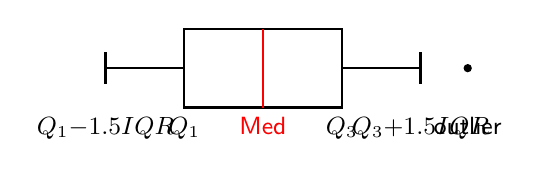
\begin{tikzpicture}[font=\sffamily\small]
        % box
        \draw[thick] (2,0) rectangle (4,1);
        % median
        \draw[thick,red] (3,0) -- (3,1);
        % whiskers
        \draw[thick] (1,0.5) -- (2,0.5);
        \draw[thick] (4,0.5) -- (5,0.5);
        % whisker caps
        \draw[thick] (1,0.3) -- (1,0.7);
        \draw[thick] (5,0.3) -- (5,0.7);
        % outlier
        \fill (5.6,0.5) circle (1.5pt);
        % labels
        \node[below] at (1,0) {\small $Q_1{-}1.5\text{IQR}$};
        \node[below] at (2,0) {\small $Q_1$};
        \node[below,red] at (3,0) {\small Med};
        \node[below] at (4,0) {\small $Q_3$};
        \node[below] at (5,0) {\small $Q_3{+}1.5\text{IQR}$};
        \node[below] at (5.6,0) {\small outlier};
    \end{tikzpicture}
\captionof{figure}{Descriptive Statistics: Five-Number Summary \& Box Plot.}
\label{fig:ch04-data-analytics-inline-01}
    \end{center}
\end{tcbitemize}

% ---- 4.2.2 Data Visualization -----------------------------------------------------------------------
\subsection{Data Visualization Techniques}

\begin{tcbitemize}[ skin=sectionraster ]
    \tcbitem[title=Chart Selection Guide, raster multicolumn=3]
    Choosing the right chart type is the first step in effective communication\textsuperscript{\cite{brucePracticalStatisticsData2017}}.
    \tcblower
    \begin{tblr}{colspec={|X|X|}, hlines}
        \textbf{Goal}               & \textbf{Recommended chart} \\
        Distribution of one variable & Histogram, KDE, box plot, violin \\
        Two-variable relationship    & Scatter plot, bubble chart \\
        Composition / proportions    & Pie (few slices), stacked bar \\
        Ranking / comparison         & Bar chart (sort by value) \\
        Trend over time              & Line chart \\
        Correlation matrix           & Heatmap \\
        High-dimensional overview    & Pair plot, parallel coordinates \\
    \end{tblr}
\captionof{table}{Data Visualization Techniques: Chart Selection Guide.}
\label{tab:ch04-data-analytics-inline-23}

    \tcbitem[title=Principles of Effective Visualization, raster multicolumn=3]
    Good visualizations maximize the \emph{data-ink ratio}: remove all ink that does not represent data\textsuperscript{\cite{brucePracticalStatisticsData2017}}.
    \tcblower
    \begin{itemize}
        \item \textbf{Tufte's rule}: erase non-data ink; avoid chartjunk (3-D effects, unnecessary gridlines)
        \item \textbf{Preattentive attributes}: position, color, size are processed instantly; use them for key encodings
        \item \textbf{Aspect ratio}: choose a ratio that highlights the trend; the ``banking to 45°'' guideline for line charts
        \item \textbf{Color}: use perceptually uniform colormaps (viridis, cividis) for continuous data; categorical palettes for discrete groups
        \item \textbf{Annotation}: label the key finding directly on the chart, not only in the caption
    \end{itemize}
\end{tcbitemize}

% ---- 4.2.3 Correlation Analysis ---------------------------------------------------------------------
\subsection{Correlation Analysis}

\begin{tcbitemize}[ skin=sectionraster ]
    \tcbitem[title=Pearson Correlation, raster multicolumn=3]
    Pearson's $r$ measures the strength and direction of the \emph{linear} relationship between two continuous variables\textsuperscript{\cite{brucePracticalStatisticsData2017}}.
    \begin{equation}
        r = \frac{\sum_{i=1}^n (x_i - \bar{x})(y_i - \bar{y})}{\sqrt{\sum_i (x_i-\bar{x})^2}\sqrt{\sum_i (y_i-\bar{y})^2}}
    \end{equation}
    Range: $r \in [-1, 1]$. $|r| = 1$ indicates perfect linear relationship; $r = 0$ indicates no \emph{linear} relationship (but nonlinear dependence may still exist).

    \tcbitem[title=Spearman Rank Correlation, raster multicolumn=3]
    Spearman's $\rho$ is a non-parametric alternative: it computes Pearson's $r$ on the \emph{ranks} of the data\textsuperscript{\cite{brucePracticalStatisticsData2017}}.
    It is robust to outliers and monotone non-linear relationships.
    \begin{equation}
        \rho = 1 - \frac{6\sum_i d_i^2}{n(n^2-1)}
    \end{equation}
    where $d_i$ is the difference in ranks for observation $i$.
    Preferred over Pearson when data is ordinal or heavy-tailed.

    \tcbitem[title={Correlation Matrix \& Correlation Is Not Causation}, raster multicolumn=6]
    A \emph{correlation matrix} displays pairwise correlations for all variable pairs simultaneously; a heatmap visualization quickly reveals clusters of correlated features\textsuperscript{\cite{brucePracticalStatisticsData2017}}.

    \textbf{Correlation does not imply causation.} Three alternative explanations always exist for a correlation between $X$ and $Y$:
    \tcblower
    \begin{tblr}{colspec={|Q[l,m,3cm]|X|}, hlines}
        \textbf{Explanation}         & \textbf{Example} \\
        $X$ causes $Y$                & Ice cream sales $\to$ drownings? (no) \\
        $Y$ causes $X$               & Reverse causation \\
        Confounding variable $Z$      & Hot weather increases both ice cream \emph{and} swimming \\
        Spurious correlation          & Nicolas Cage films $\sim$ pool drownings (coincidence) \\
    \end{tblr}
\captionof{table}{Correlation Analysis: Correlation Matrix \& Correlation Is Not Causation.}
\label{tab:ch04-data-analytics-inline-24}
    Establishing causation requires randomized controlled trials (RCTs) or causal inference methods (Pearl's do-calculus, instrumental variables, regression discontinuity).
\end{tcbitemize}

% ---- 4.2.4 Dimensionality Reduction -----------------------------------------------------------------
\subsection{Dimensionality Reduction}

\begin{tcbitemize}[ skin=sectionraster ]
    \tcbitem[title={PCA Step-by-Step}, raster multicolumn=3]
    Principal Component Analysis finds a lower-dimensional linear subspace that captures maximum variance\textsuperscript{\cite{hastieElementsStatisticalLearning2008}}.
    \tcblower
    \begin{enumerate}
        \item \textbf{Center} the data: subtract the column means so $\mathbb{E}[\mathbf{X}] = \mathbf{0}$
        \item (Optionally \textbf{scale}: divide by column std to get unit variance)
        \item \textbf{Compute} the covariance matrix $\mathbf{C} = \frac{1}{n-1}\mathbf{X}^\top\mathbf{X}$
        \item \textbf{Eigendecompose}: $\mathbf{C} =
              \mathbf{V}\boldsymbol{\Lambda}\mathbf{V}^\top$; columns of
              $\mathbf{V}$ are principal directions
        \item \textbf{Sort} eigenvectors by descending eigenvalue $\lambda_1 \geq \lambda_2 \geq \cdots$
        \item \textbf{Project}: $\mathbf{Z} = \mathbf{X}\mathbf{V}_k$ retains the top-$k$ components
        \item \textbf{Explained variance ratio}: $\frac{\lambda_j}{\sum_i \lambda_i}$; choose $k$ so cumulative ratio $\geq$ 95\%
    \end{enumerate}

    \tcbitem[title={t-SNE \& UMAP}, raster multicolumn=3]
    For high-dimensional data, linear PCA often fails to reveal cluster structure visible to non-linear methods\textsuperscript{\cite{hastieElementsStatisticalLearning2008}}.
    \tcblower
    \textbf{t-SNE} (van der Maaten \& Hinton, 2008):
    \begin{itemize}
        \item Models pairwise similarities as Gaussians in high-D, Student-$t$ in low-D
        \item Minimizes KL divergence between the two distributions via gradient descent
        \item Preserves local structure extremely well; global distances not preserved
        \item Stochastic; different runs give different layouts; use for visualization only
    \end{itemize}
    \textbf{UMAP} (McInnes et al., 2018):
    \begin{itemize}
        \item Fuzzy topological data analysis; builds and aligns $k$-nearest-neighbor graphs
        \item Faster than t-SNE; better global structure preservation
        \item Supports new-point embedding (transform); useful for pipelines
    \end{itemize}
\end{tcbitemize}

\section{Literature}
\begin{itemize}
    \item Han, J., Kamber, M., \& Pei, J. (2011). Data mining: Concepts and techniques (3rd ed.). Morgan Kaufmann.
    \item Provost, F., \& Fawcett, T. (2013). Data science for business: What you need to know about data mining and data-analytic thinking. O'Reilly Media.
    \item Tukey, J. W. (1977). Exploratory data analysis. Addison-Wesley.
    \item Andrade, H., Gedik, B., \& Turaga, D. (2014). Fundamentals of stream processing: Application
          design, systems, and analytics. Cambridge University Press.
    \item Axelrod, C. W. (2013). Engineering safe and secure software systems. Artech House.
    \item Kleppmann, M. (2017). Designing data-intensive applications: The big ideas behind reliable,
          scalable, and maintainable systems. O'Reilly.
    \item Newman, S. (2015). Building microservices: Designing fine-grained systems. O'Reilly.
\end{itemize}
